\newpage
\section{Экспериментальное исследование}

\subsection{Общие замечания}

Для исследования предложенного в \cref{section:dangling} алгоритма и сравнения его с иными
подходами, такими как мгновенное удаление запрошенных элементов и, как следствие, отсутствие
мусора в системе, был написан прототип на языке Go.

Был исследован сценарий, типичный для поисковых систем, когда в индексе добавляется большое
количество документов $N_0$, затем удаляется $N_0\cdot \lambda$, где $\lambda \in [0; 1]$.

Пороговое значение \textit{dangling} для индексе устанавливается
$\frac{\text{bitmap block size} \cdot \lambda}{C}$, где $C \in \mathbb{I}, C \leq 2$ для
большого накопления мусора.

Для этого сценария были изучены производительность таких операций, как:
\begin{enumerate}
    \item Измерение времени поиска признаков до фактического удаления элементов.
    Как следствие, множество ненужных обращений к памяти для \textit{повисших}
    документов.
    \item Измерение времени поиска признаков после сбора мусора.
    \item Измерение времени поиска признаков после <<мгновенного удаления>>.
    \item Измерение времени работы алгоритма сбора мусора и алгоритма <<мгновенного удаления>>.
\end{enumerate}

Каждый вариант поиска признаков разбивается на 2 варианта:
\begin{enumerate}
      \item Запрос по всем вхождениям заданного ключа для фиксированного числа
      добавленных элементов $N_0$ и меняющегося размера блока битмапы $2^{x}$.
      \item Запрос по первому вхождению заданного ключа для фиксированного числа
      добавленных элементов $N_0$ и меняющегося размера блока битмапы $2^{x}$.
      \item Измерение времени поиска всех вхождения признака для меняющегося числа добавленных элементов $N_0$.
\end{enumerate}

Количество добавленных документов $N_0 = 10^{x}, x \in \{2, \cdots, 6\}$ в нашем опыте.
Измеряется время поиска признаков с различной частотой появления в индексе: 1,
5, 10, 15\%, от общего числа добавленных документов.

%Далее при различных размерах блока, тем самым выясняется оптимальный размер блока. В реальности это значение получается из логических соображений (ни много, ни мало) и колеблется около 15\%.

Кроме того, для предложенного индекса была изучена зависимость количества чтений,
записей на диск и слияний с данными на диске после добавления элементов и после
их удаления в зависимости от количества добавленных элементов $N_0$.

\begin{table}[H]
\caption{Аппаратные и программные характеристики платформы}
\centering
\small
\singlespacing
\begin{tabular}{|c|c|}
      \hline
      Тип накопителя         & HDD              \\ \hline
      Архитектура процессора & x86-64           \\ \hline
      Частота процессора     & $2.60$ ГГц       \\ \hline
      Количество ядер        & 4                \\ \hline
      Оперативная память     & 28.90 Гб         \\ \hline
      L2 кэш                 & 1024 Кб          \\ \hline
      Операционная система   & Ubuntu 18.04 LTS \\ \hline
      Компилятор             & Go 1.13.8        \\ \hline
\end{tabular}
\label{tab:arch_settings}
\end{table}

\begin{table}[H]
      \caption{Настройки индекса}
      \centering
      \small
      \singlespacing
      \begin{tabular}{|l|c|}
            \hline
            Кеш                                                                           & $2\cdot 1024\cdot 1024$ байт \\ \hline
            Соотношение размеров соседних уровней                                         & 10               \\ \hline
            Задержка при записи                                                           & 50 мс            \\ \hline
            Задержка при чтении                                                           & 20 мс            \\ \hline
            Отношение числа удаленных документов к добавленным $\lambda$                  & $\frac{2}{3}$    \\ \hline
            Пороговое отношение числа \textit{повисших} документов $\frac{\lambda}{C}$    & $\frac{1}{3}$    \\ \hline
\end{tabular}
\label{tab:lsm_settings}
\end{table}

Сравним производительность индекса после добавления $10^2$, $10^3$, $10^4$ и $10^5$
документов соответственно. Для каждого значения добавленных элементов рассмотрим
признаки с различающейся частотой повторения в данных.

\subsection{Поисковый запрос по всем вхождениям заданного ключа для фиксированного числа добавленных элементов}

\subsubsection{Добавление $10^3$ документов}

\begin{figure}[H]
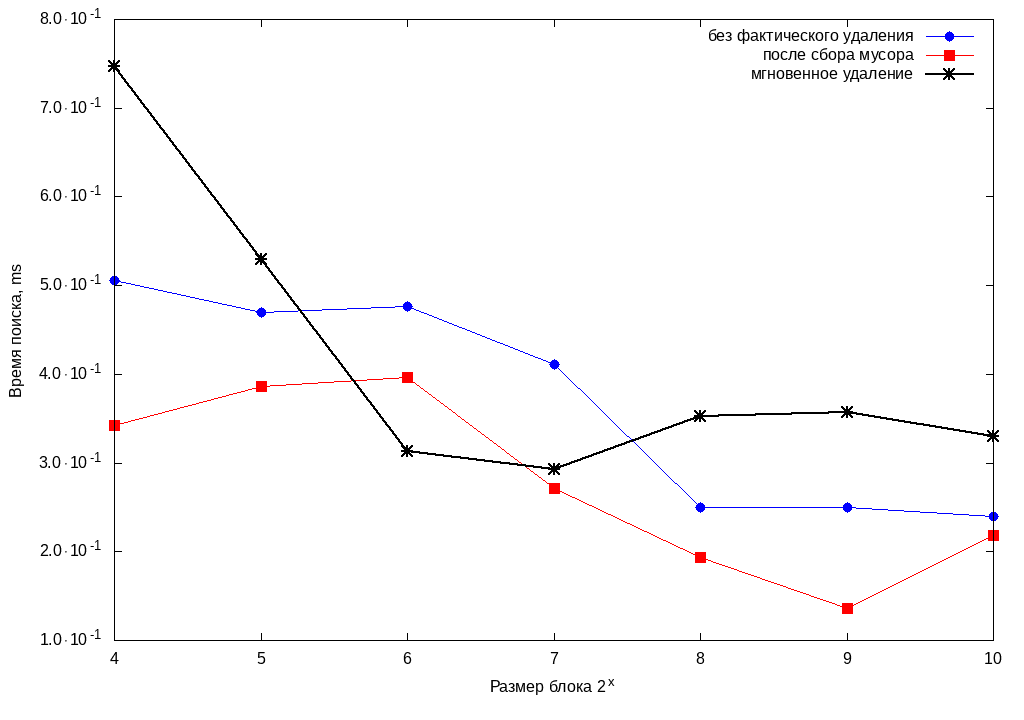
\includegraphics[width=\linewidth, height=10cm]{fig/limit_1e6/1e3/body.png}
\caption{Признак \textit{body} встречается в 16\% документов}
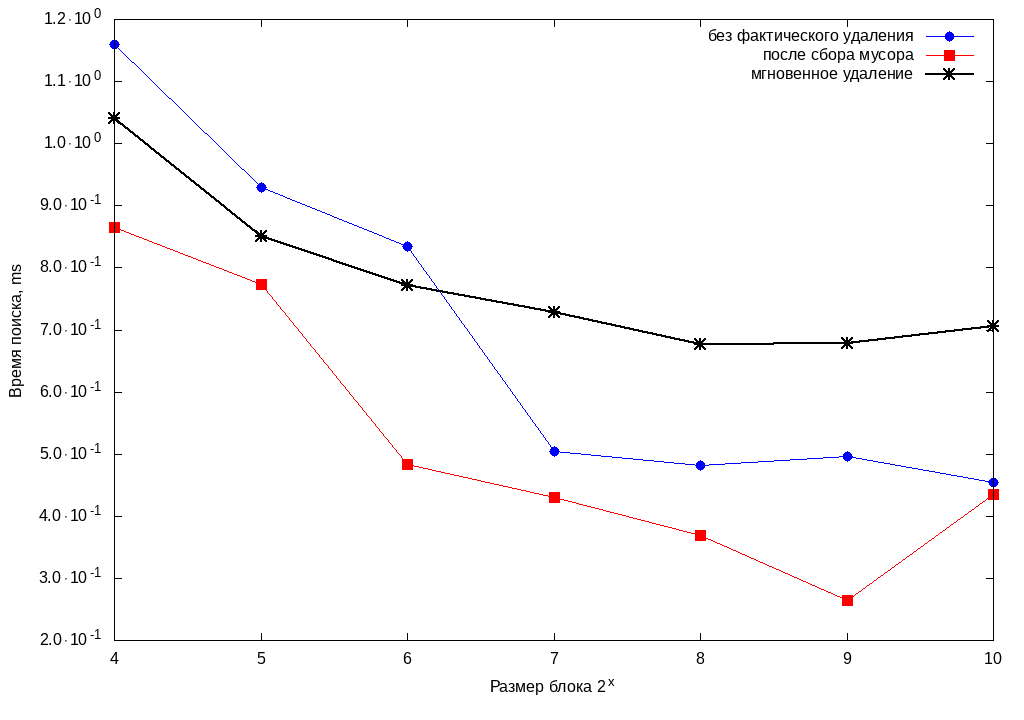
\includegraphics[width=\linewidth, height=11cm]{fig/limit_1e6/1e3/from.png}
\caption{Признак \textit{from} встречается в 31\% документов}
\end{figure}

\begin{figure}[H]
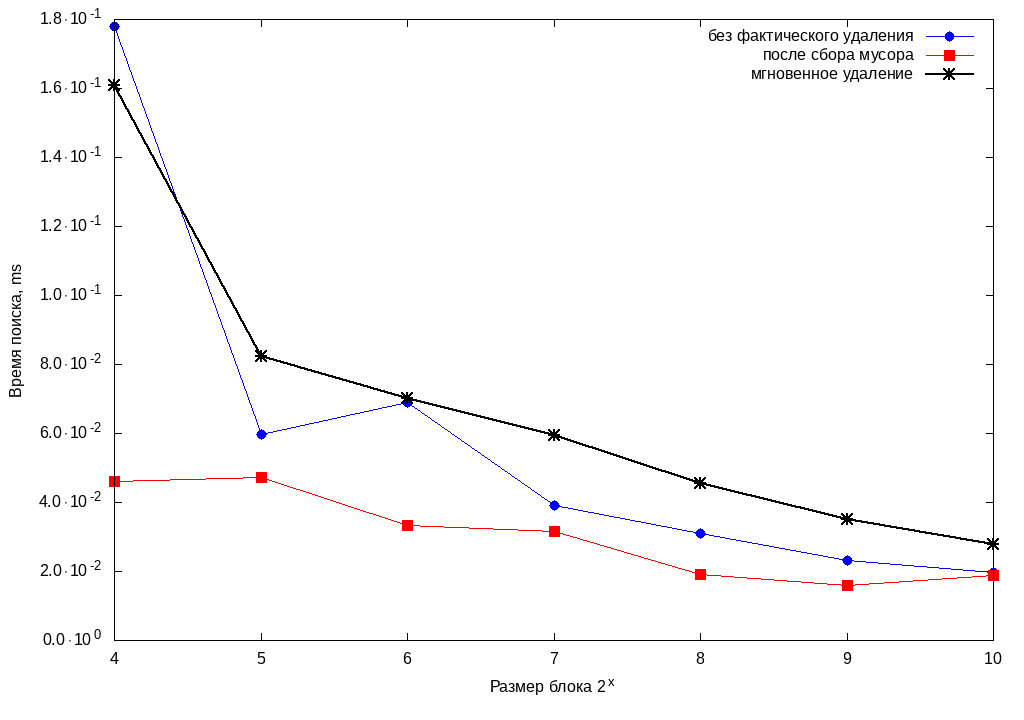
\includegraphics[width=\linewidth, height=11cm]{fig/limit_1e6/1e3/to.png}
\caption{Признак \textit{to} встречается менее, чем в 1\% документов}
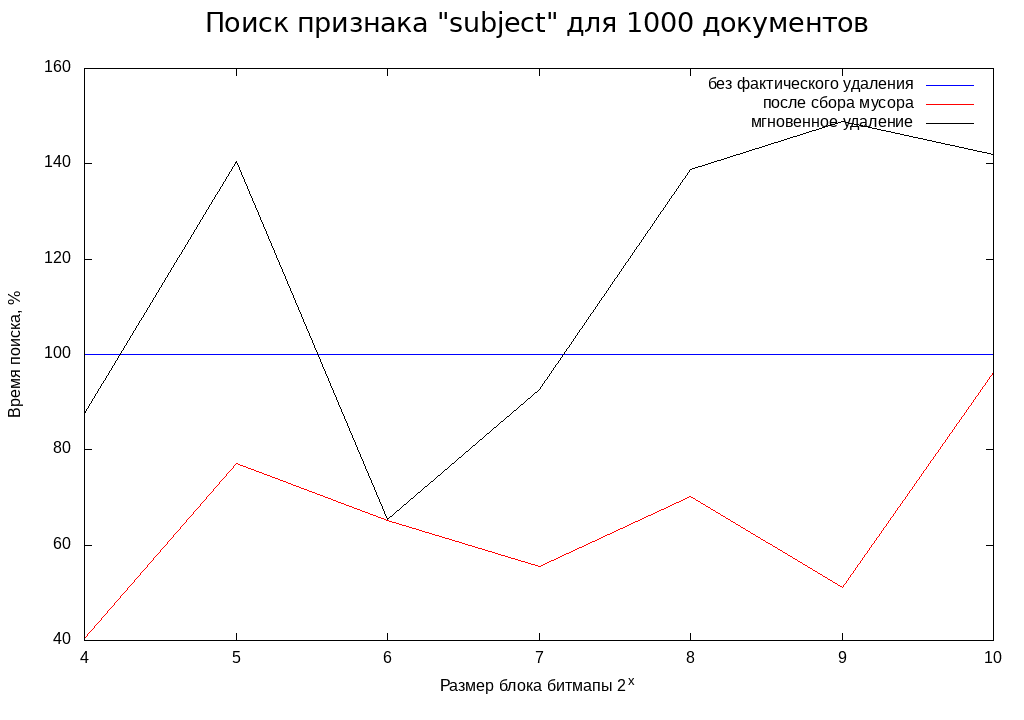
\includegraphics[width=\linewidth, height=11cm]{fig/limit_1e6/1e3/subject.png}
\caption{Признак \textit{subject} встречается в 13\% документов}
\end{figure}

\textbf{Вывод}: для $10^3$ элементов алгоритм сбора мусора дает существенный
прирост в скорости поиска по сравнению с <<мгновенным>> удалением и поиском в данных с мусором.

\subsubsection{Добавление $10^4$ документов}

\begin{figure}[H]
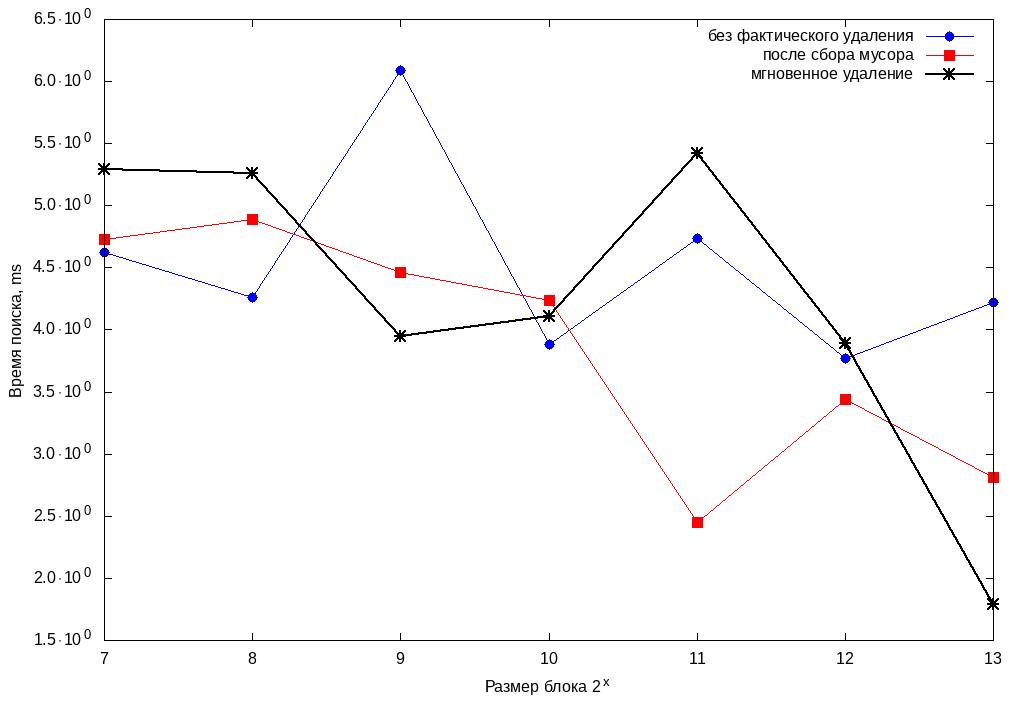
\includegraphics[width=\linewidth, height=10cm]{fig/limit_1e6/1e4/body.png}
\caption{Признак \textit{body} встречается в 18\% документов}
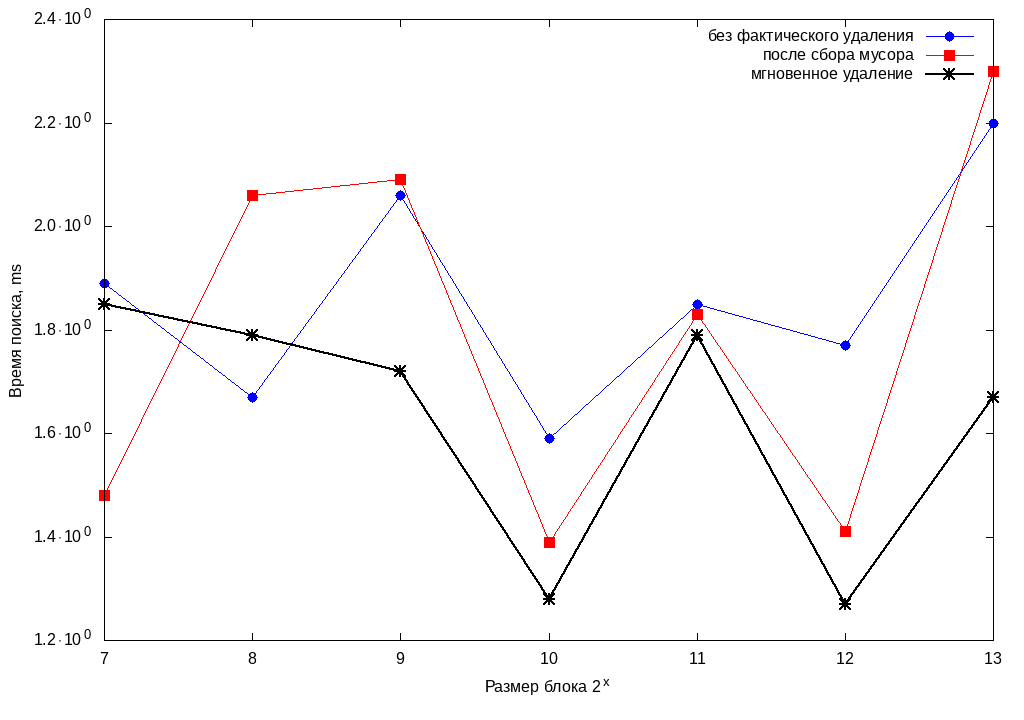
\includegraphics[width=\linewidth, height=11cm]{fig/limit_1e6/1e4/from.png}
\caption{Признак \textit{from} встречается в 7\% документов}
\end{figure}

\begin{figure}[H]
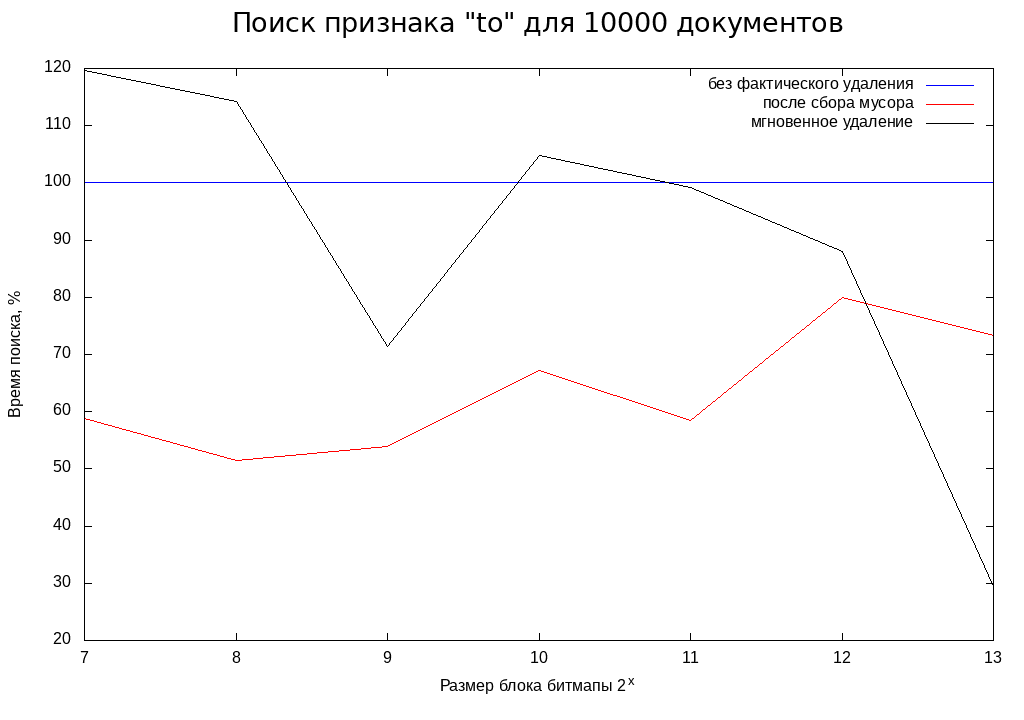
\includegraphics[width=\linewidth, height=11cm]{fig/limit_1e6/1e4/to.png}
\caption{Признак \textit{to} встречается менее, чем в 1\% документов}
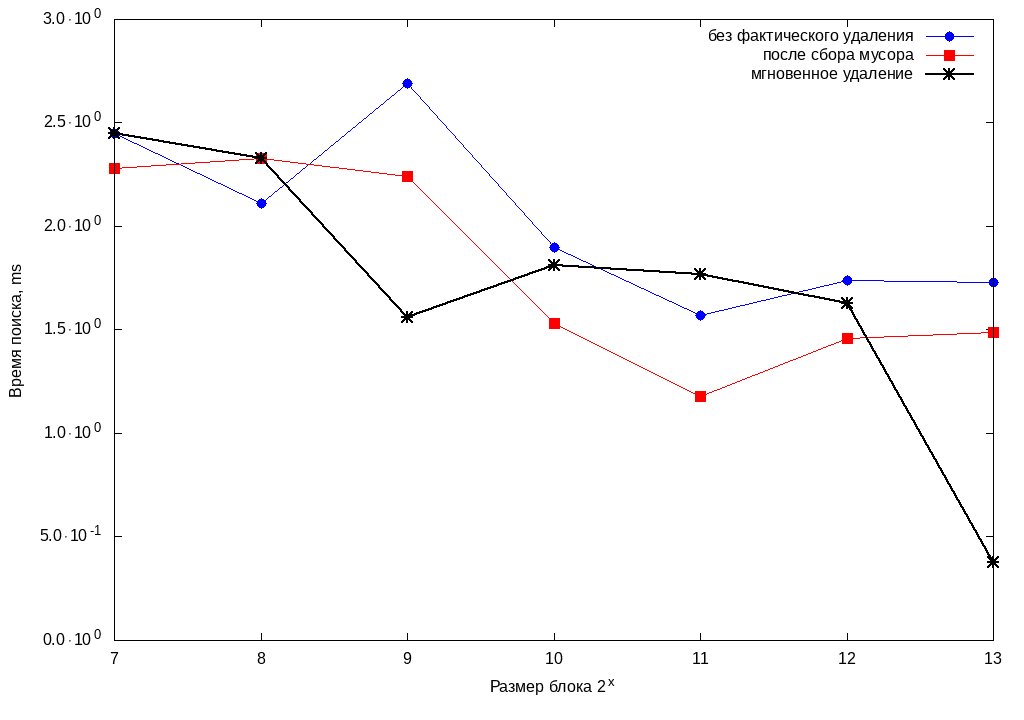
\includegraphics[width=\linewidth, height=11cm]{fig/limit_1e6/1e4/subject.png}
\caption{Признак \textit{subject} встречается в 8\% документов}
\end{figure}

\textbf{Вывод}: для $10^4$ элементов алгоритм сбора мусора дает выигрыш на большинстве признаков
по сравнению в <<мгновенным>> удалением и поиском в данных с мусором.

\subsubsection{Добавление $10^5$ документов}

\begin{figure}[H]
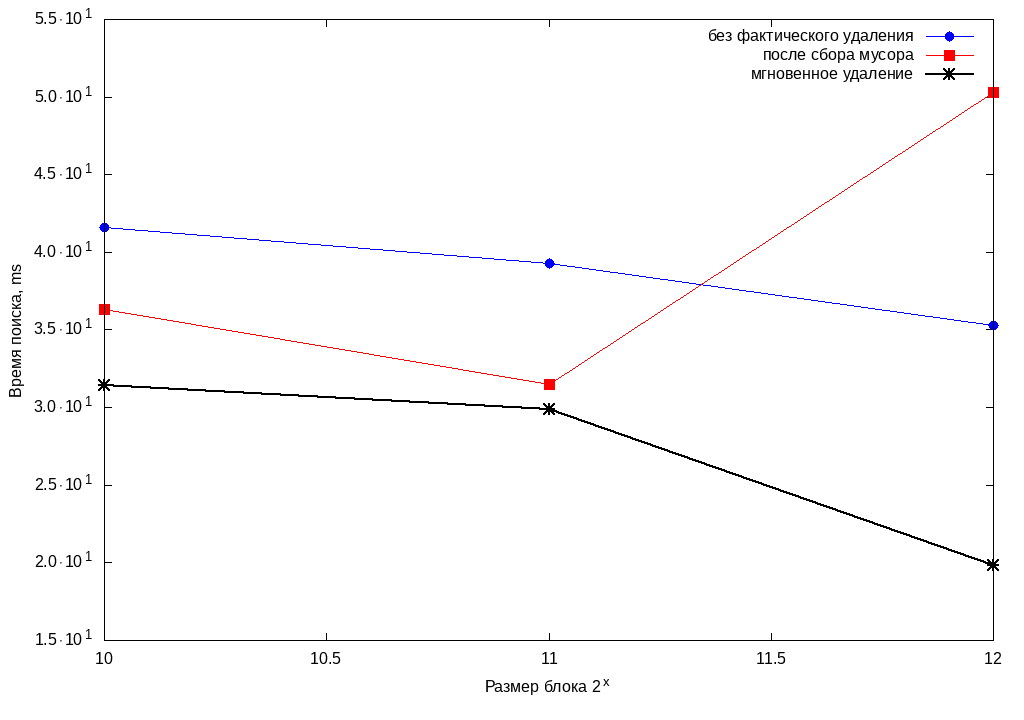
\includegraphics[width=\linewidth, height=10cm]{fig/limit_1e6/1e5/body.png}
\caption{Признак \textit{body} встречается в 16\% документов}
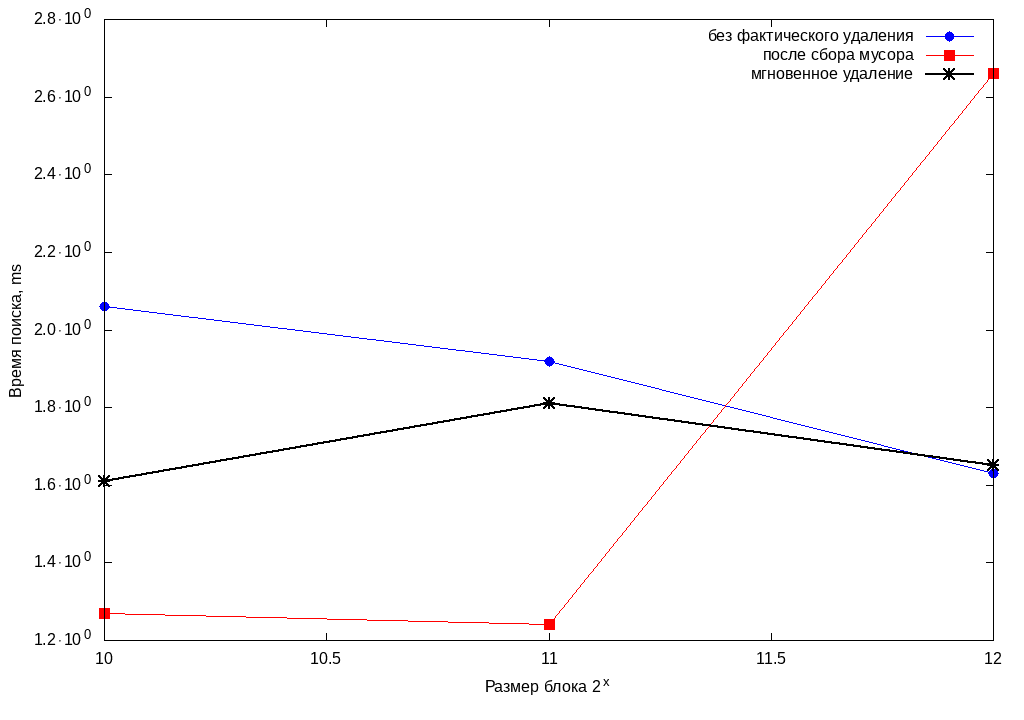
\includegraphics[width=\linewidth, height=11cm]{fig/limit_1e6/1e5/from.png}
\caption{Признак \textit{from} встречается в 1\% документов}
\end{figure}

\begin{figure}[H]
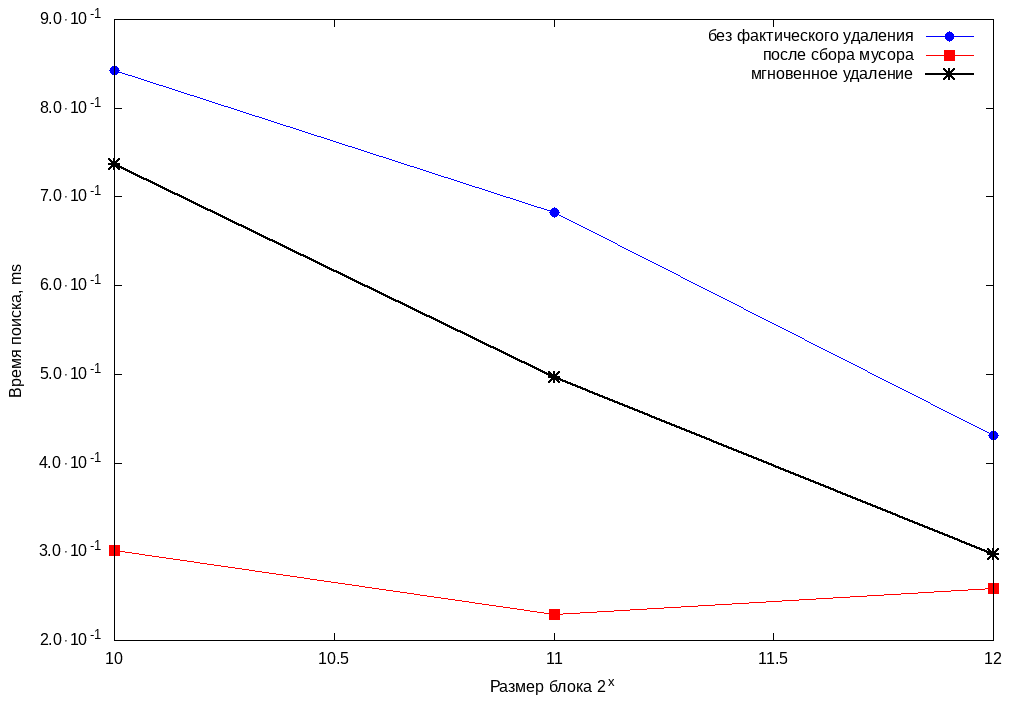
\includegraphics[width=\linewidth, height=11cm]{fig/limit_1e6/1e5/to.png}
\caption{Признак \textit{to} встречается в 0,05\% документов}
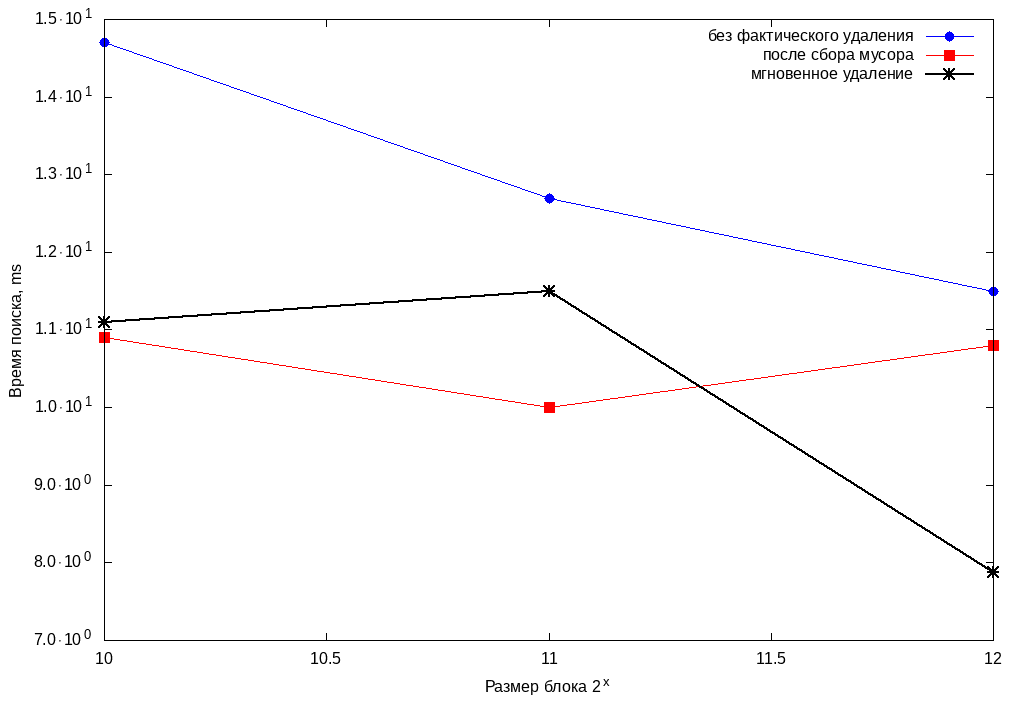
\includegraphics[width=\linewidth, height=11cm]{fig/limit_1e6/1e5/subject.png}
\caption{Признак \textit{subject} встречается в 5\% документов}
\end{figure}

\textbf{Вывод}: для $10^5$ добавленных документов алгоритм сбора мусора эффективнее
по сравнению в <<мгновенным>> удалением и поиском в данных с мусором.

\subsection{Поисковый запрос по первому вхождению заданного ключа для фиксированного числа добавленных элементов}

\subsubsection{Добавление $10^3$ документов}

\begin{figure}[H]
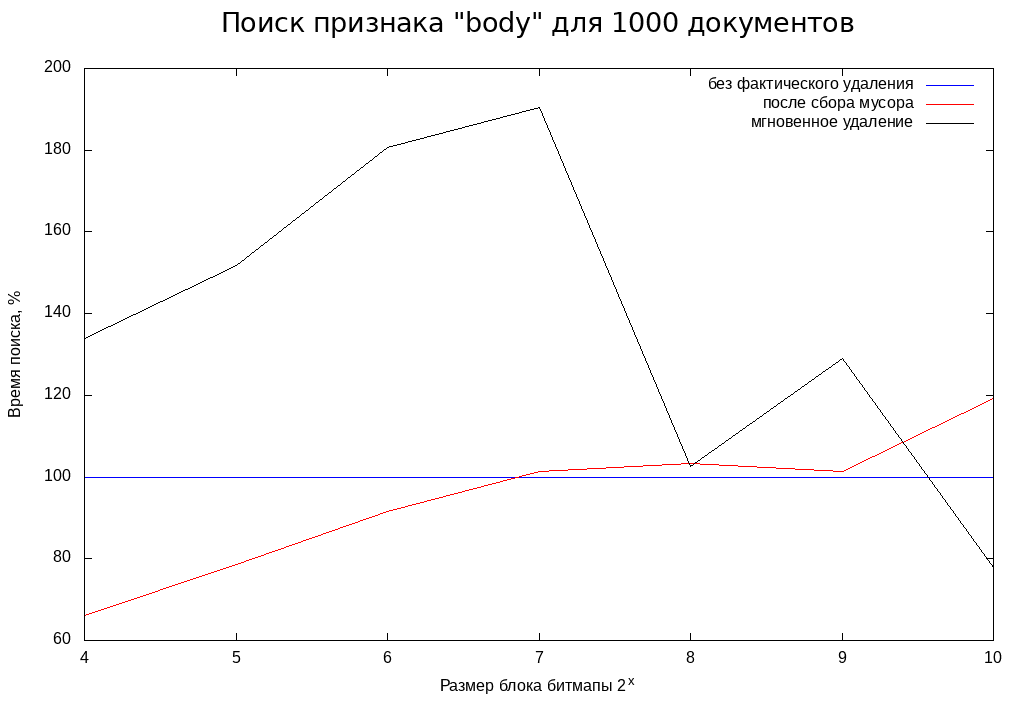
\includegraphics[width=\linewidth, height=10cm]{fig/limit_1/1e3/body.png}
\caption{Признак \textit{body} встречается в 16\% документов}
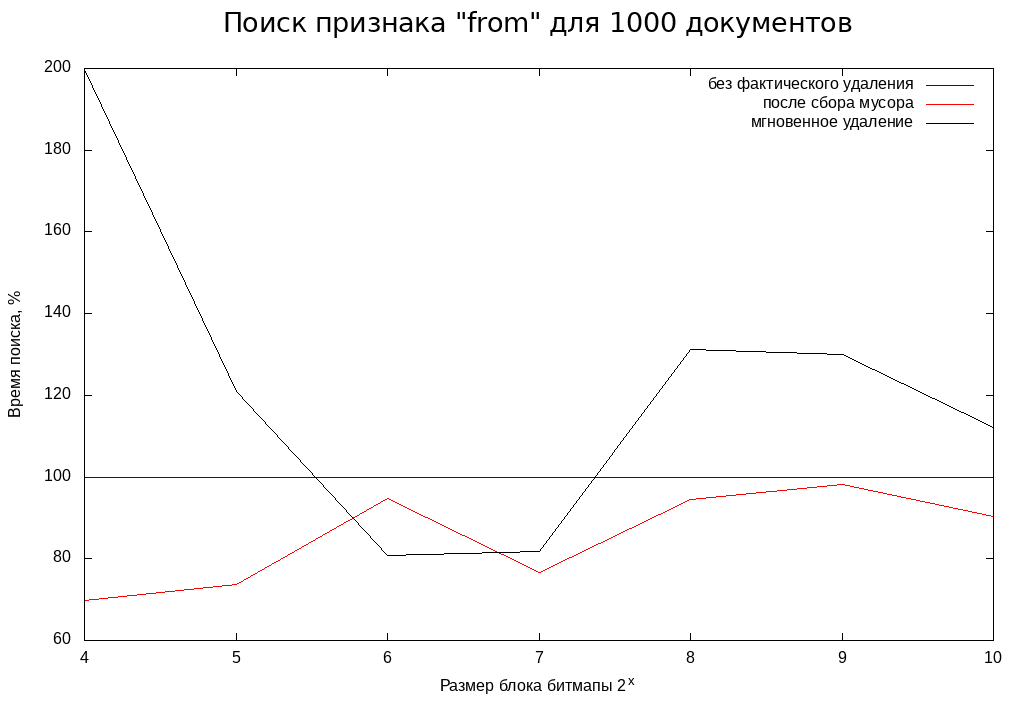
\includegraphics[width=\linewidth, height=11cm]{fig/limit_1/1e3/from.png}
\caption{Признак \textit{from} встречается в 31\% документов}
\end{figure}

\begin{figure}[H]
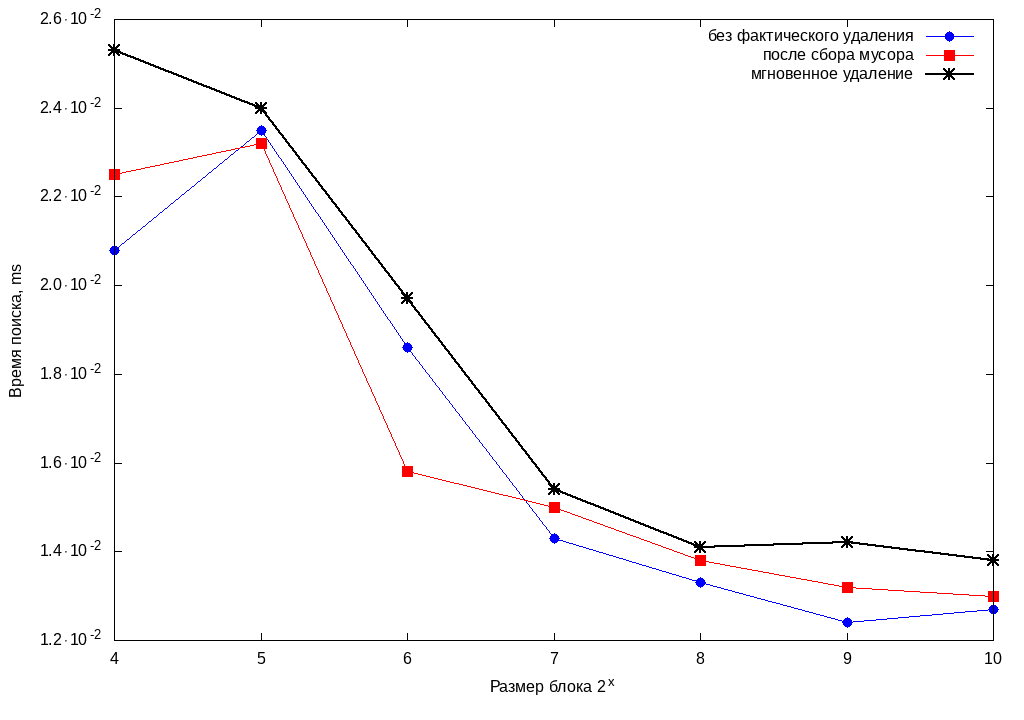
\includegraphics[width=\linewidth, height=11cm]{fig/limit_1/1e3/to.png}
\caption{Признак \textit{to} встречается менее, чем в 1\% документов}
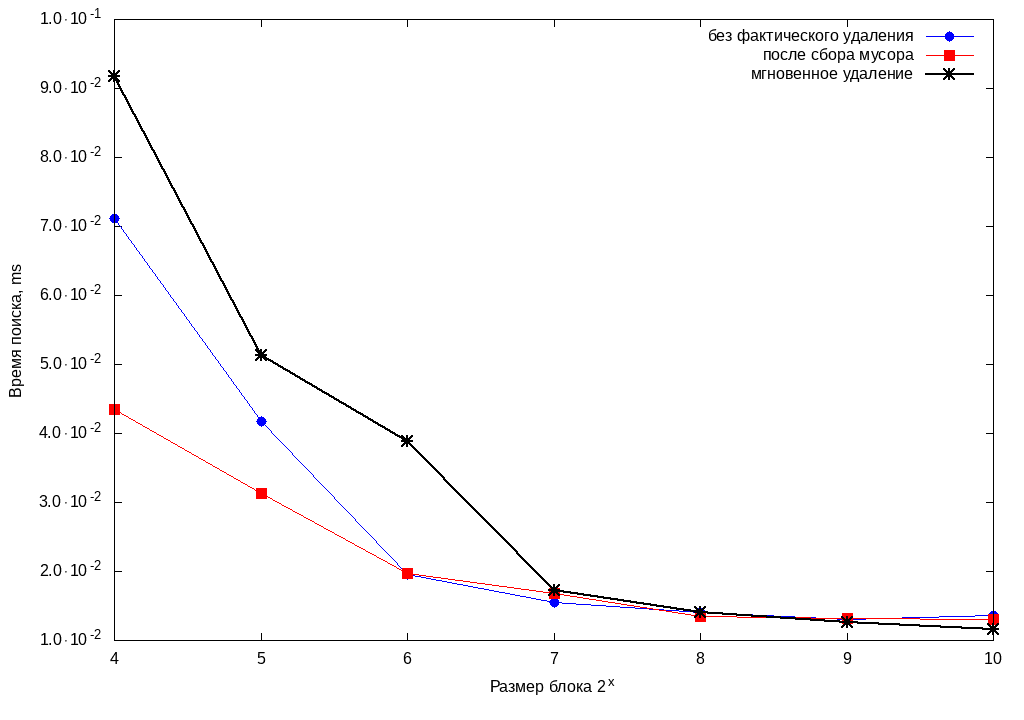
\includegraphics[width=\linewidth, height=11cm]{fig/limit_1/1e3/subject.png}
\caption{Признак \textit{subject} встречается в 13\% документов}
\end{figure}

\textbf{Вывод}: для $10^3$ элементов алгоритм <<мгновенного>> удаления и сбора мусора
не вносят существенный вклад в эффективность поиска единственного ключа.

\subsubsection{Добавление $10^4$ документов}

\begin{figure}[H]
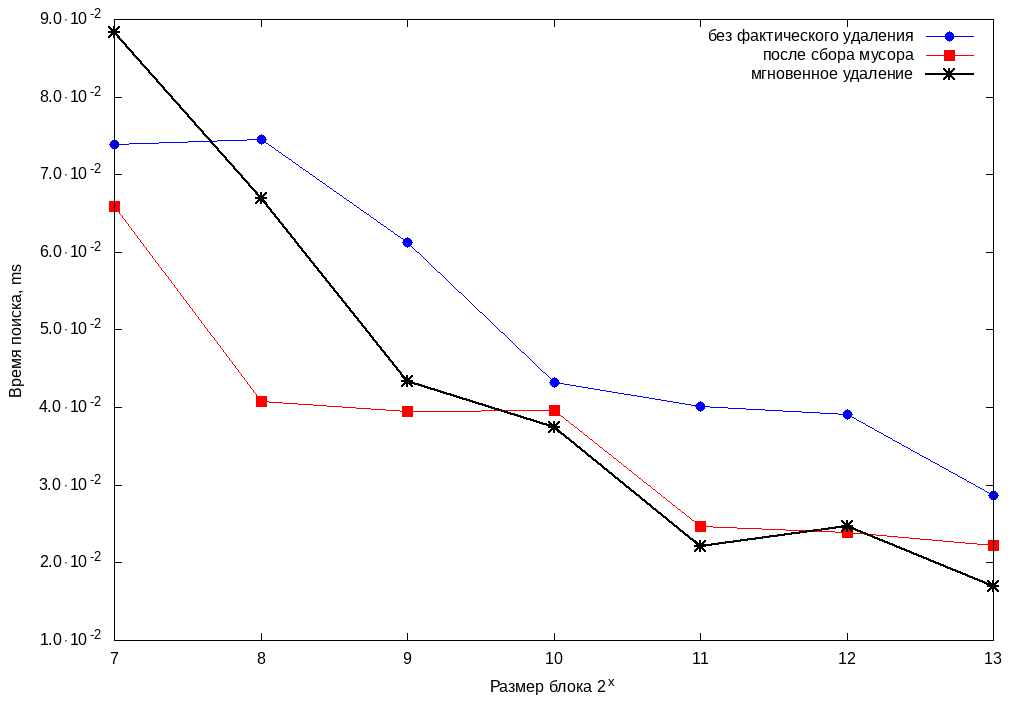
\includegraphics[width=\linewidth, height=10cm]{fig/limit_1/1e4/body.png}
\caption{Признак \textit{body} встречается в 18\% документов}
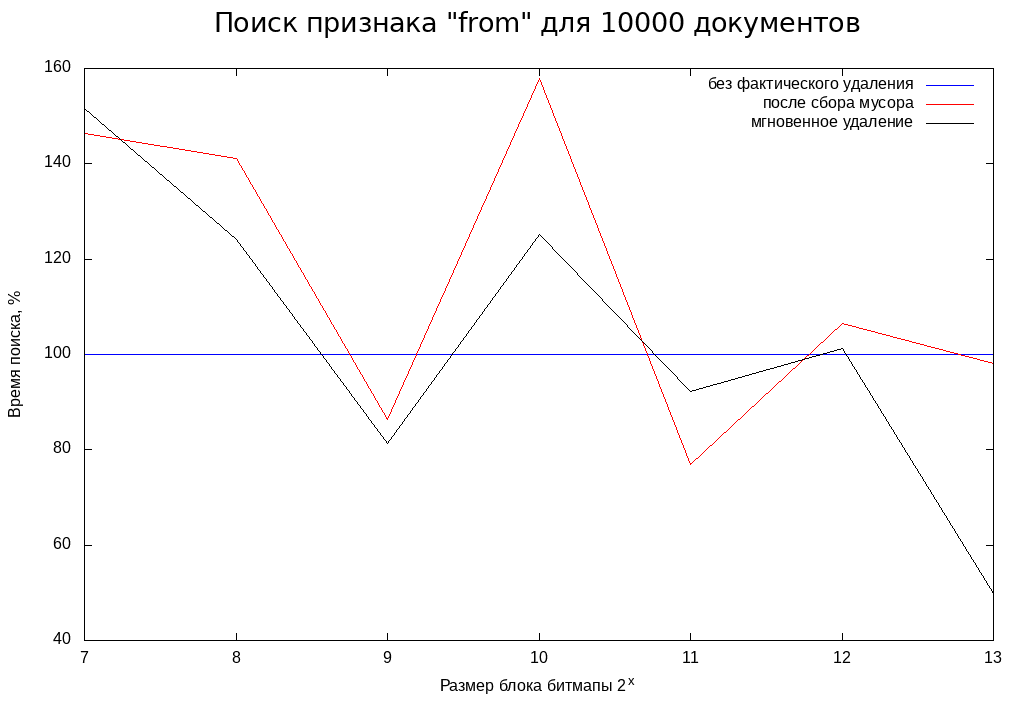
\includegraphics[width=\linewidth, height=11cm]{fig/limit_1/1e4/from.png}
\caption{Признак \textit{from} встречается в 7\% документов}
\end{figure}

\begin{figure}[H]
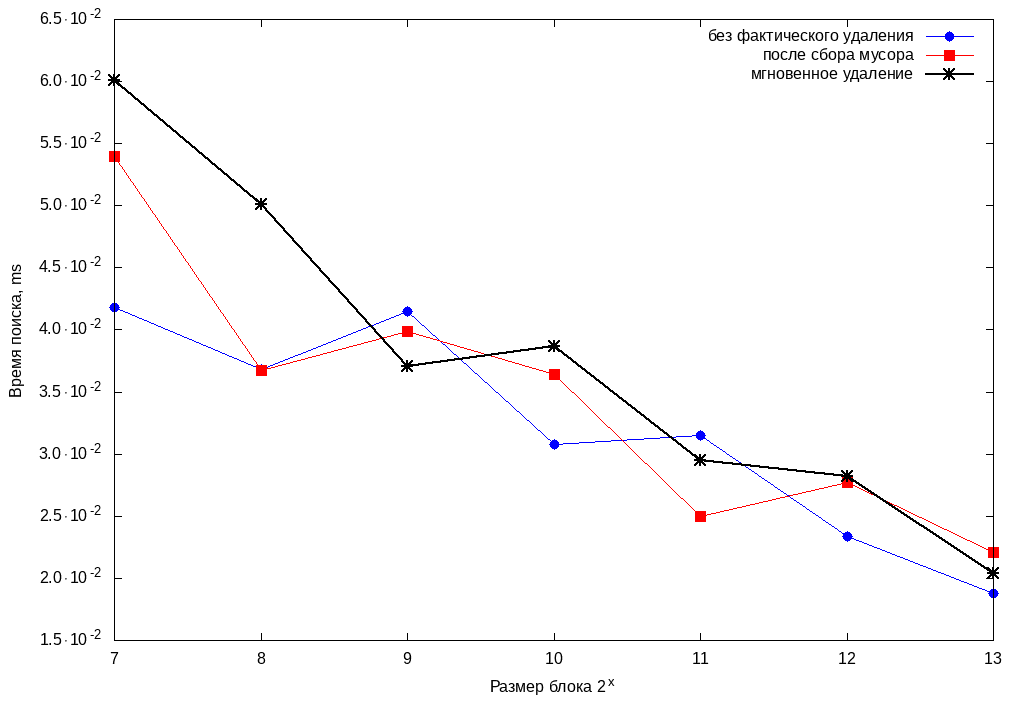
\includegraphics[width=\linewidth, height=11cm]{fig/limit_1/1e4/to.png}
\caption{Признак \textit{to} встречается менее, чем в 1\% документов}
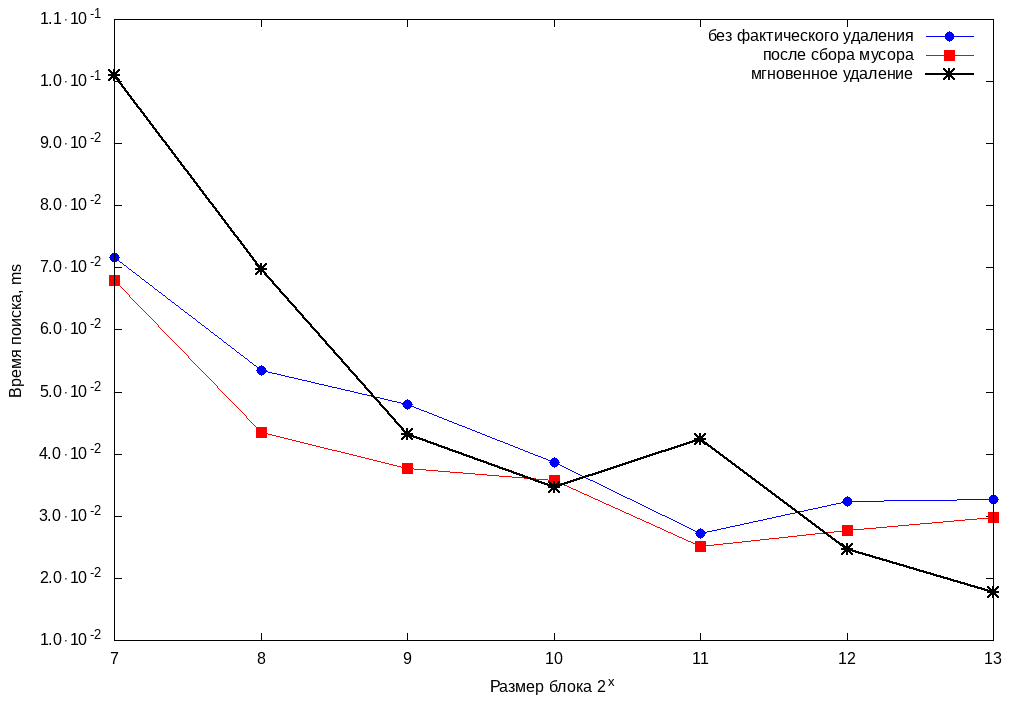
\includegraphics[width=\linewidth, height=11cm]{fig/limit_1/1e4/subject.png}
\caption{Признак \textit{subject} встречается в 8\% документов}
\end{figure}

\textbf{Вывод}: для $10^4$ элементов алгоритм сбора мусора дает выигрыш на большинстве признаков
по сравнению в <<мгновенным>> удалением и поиском в данных с мусором.

\subsubsection{Добавление $10^5$ документов}


\begin{figure}[H]
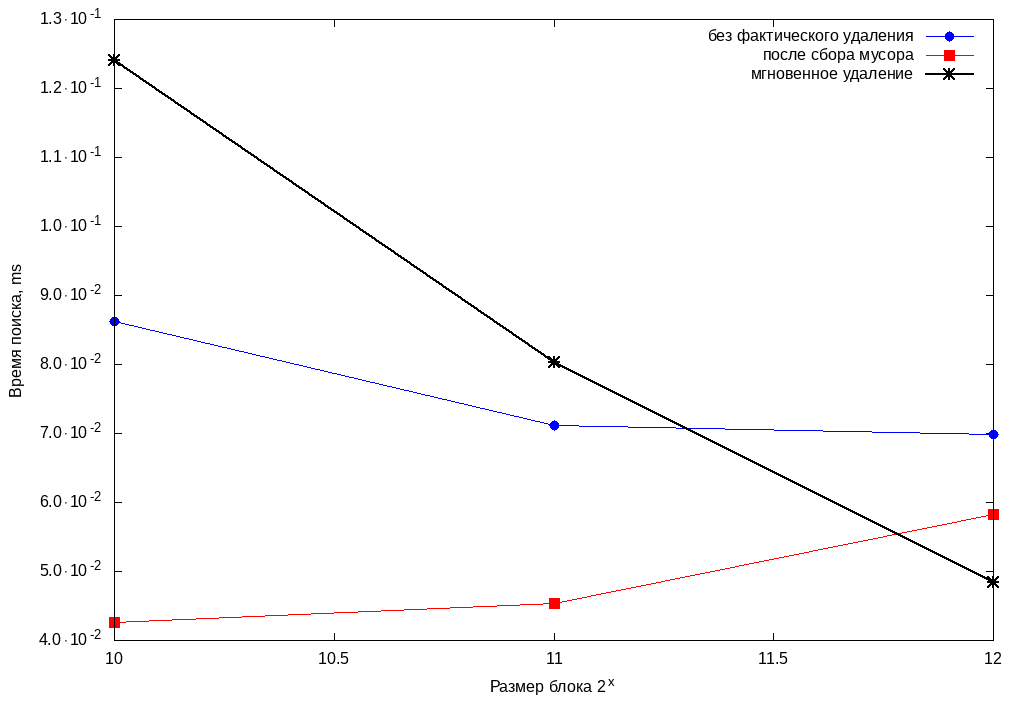
\includegraphics[width=\linewidth, height=10cm]{fig/limit_1/1e5/body.png}
\caption{Признак \textit{body} встречается в 16\% документов}
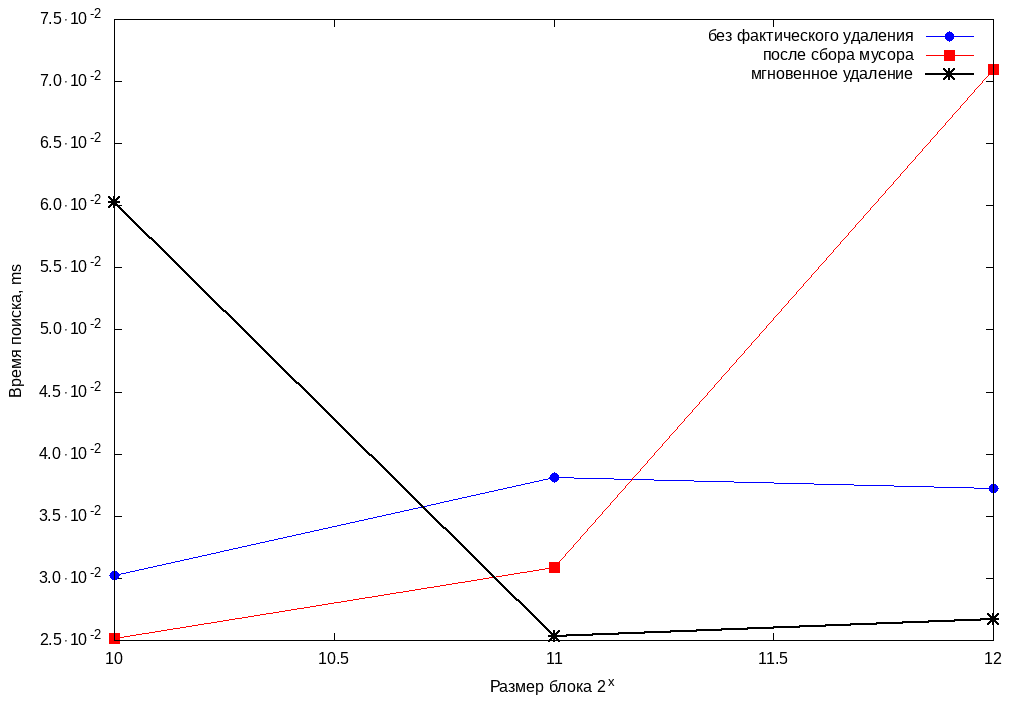
\includegraphics[width=\linewidth, height=11cm]{fig/limit_1/1e5/from.png}
\caption{Признак \textit{from} встречается в 1\% документов}
\end{figure}

\begin{figure}[H]
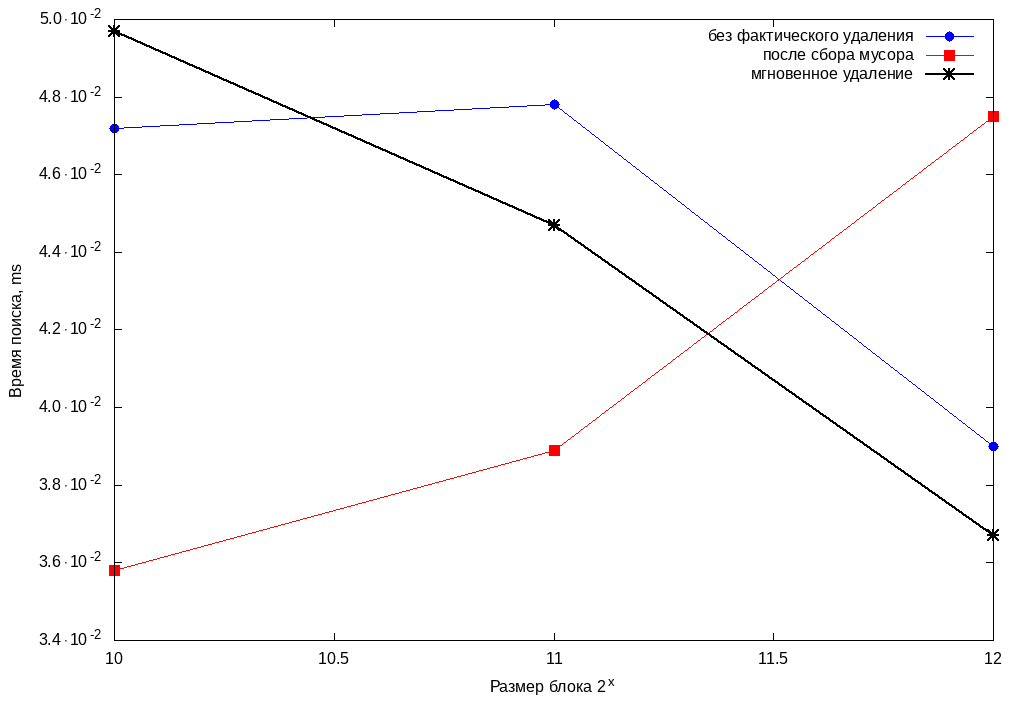
\includegraphics[width=\linewidth, height=11cm]{fig/limit_1/1e5/to.png}
\caption{Признак \textit{to} встречается в 0,05\% документов}
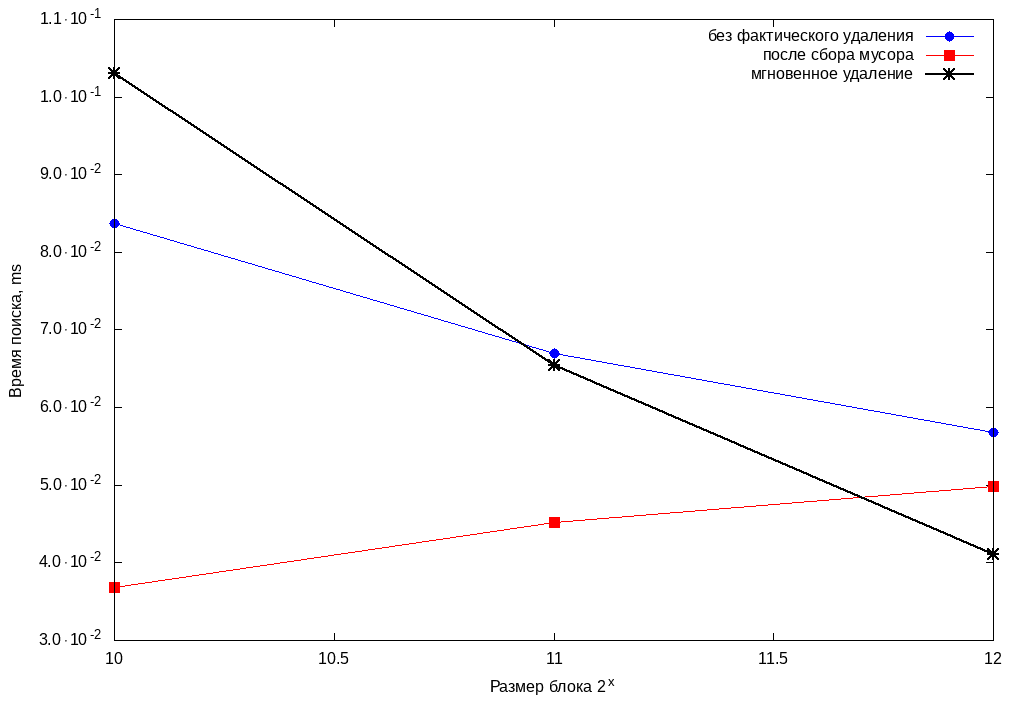
\includegraphics[width=\linewidth, height=11cm]{fig/limit_1/1e5/subject.png}
\caption{Признак \textit{subject} встречается в 5\% документов}
\end{figure}


\textbf{Вывод}: для $10^5$ добавленных документов алгоритм сбора мусора эффективнее
по сравнению в <<мгновенным>> удалением и поиском в данных с мусором.

\subsection{Сравнение времени поиска для различного числа добавленных документов}

\begin{figure}[H]
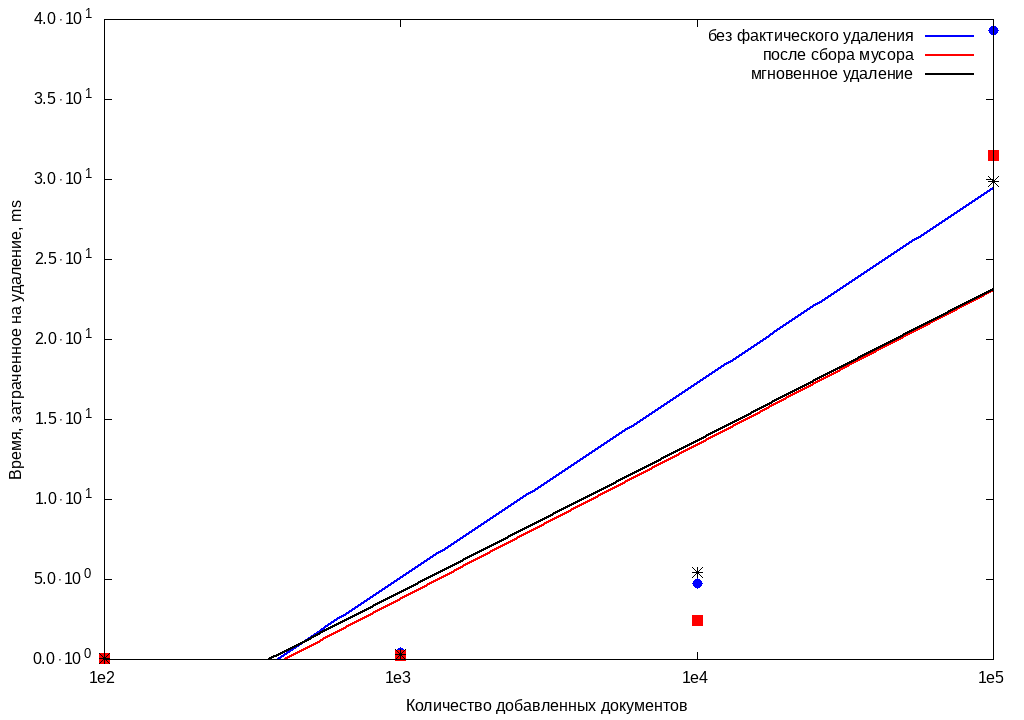
\includegraphics[width=\linewidth, height=10cm]{fig/body.png}
\caption{Признак \textit{body}}
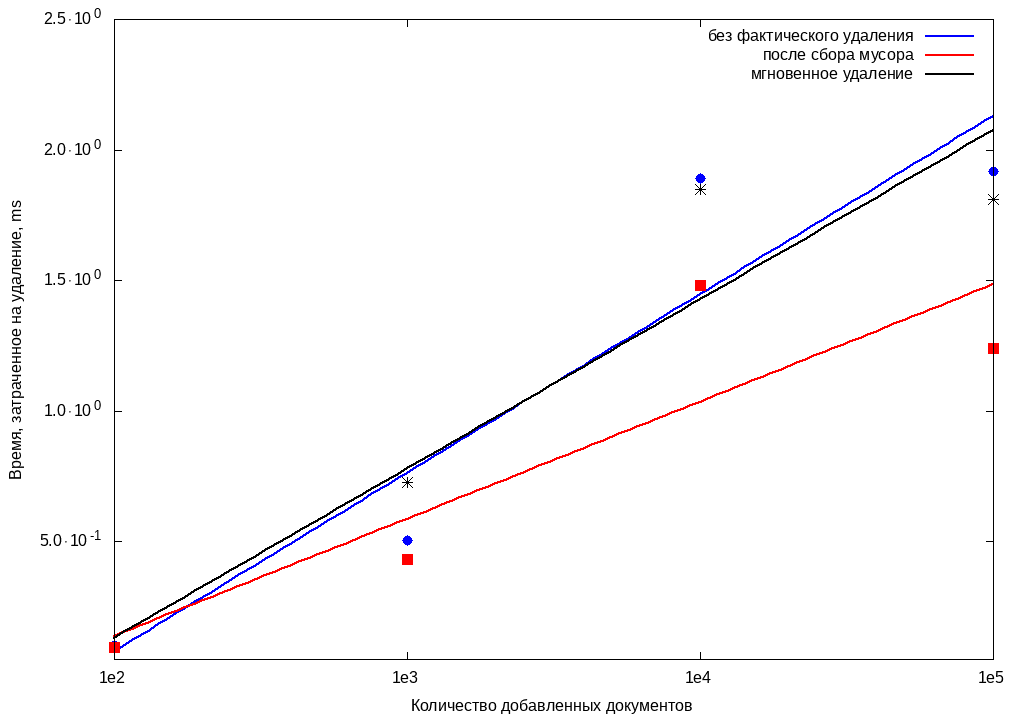
\includegraphics[width=\linewidth, height=11cm]{fig/from.png}
\caption{Признак \textit{from}}
\end{figure}

\begin{figure}[H]
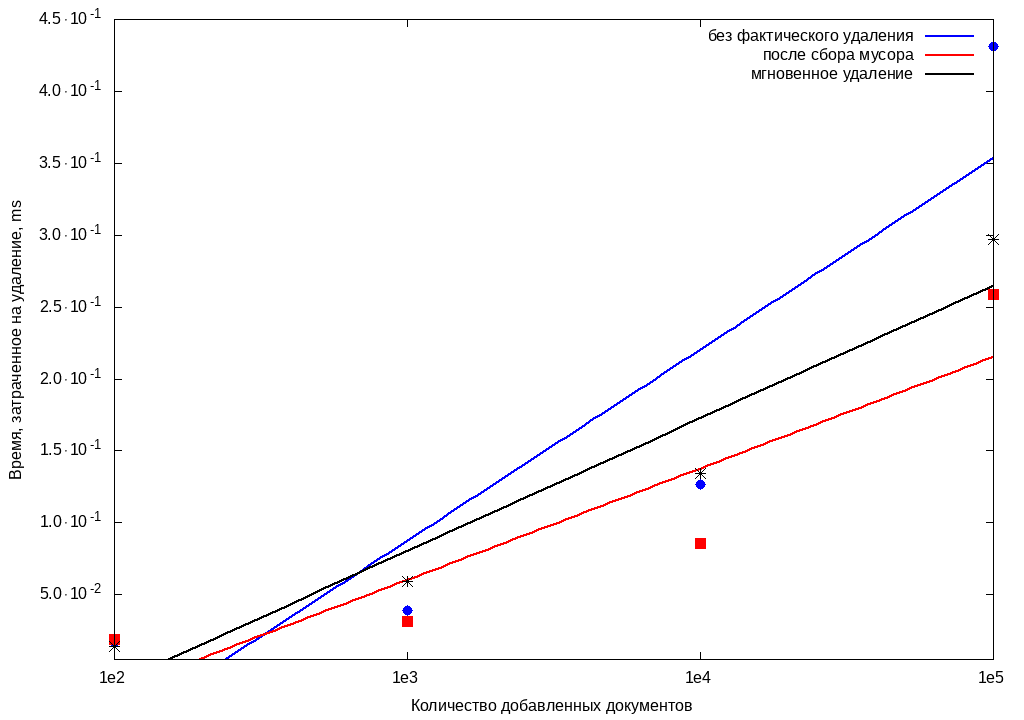
\includegraphics[width=\linewidth, height=11cm]{fig/to.png}
\caption{Признак \textit{to}}
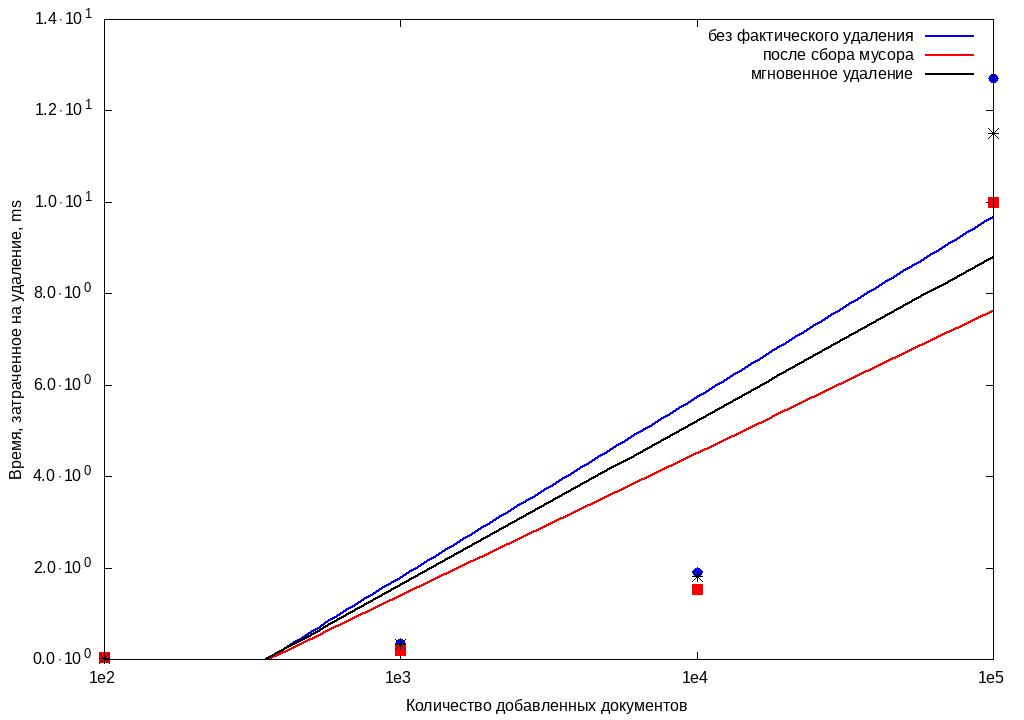
\includegraphics[width=\linewidth, height=11cm]{fig/subject.png}
\caption{Признак \textit{subject}}
\end{figure}

\textbf{Вывод}: построенная по данным модель линейной регрессии показывает
положительный тренд в плане эффективности использования сбора мусора по сравнению
с другими алгоритмами с ростом данных.

Таким образом, полученная теоретическая оценка (см. с. ~\pageref{theory})
выполняется на большинстве признаков. Погрешность вносит отличная от теоретической
разреженность битмап и меняющаяся от признака к признаку частота появления в
документах.

\newpage
\subsection{Сравнение времени работы алгоритмов для различного числа добавленных документов}

\subsubsection{Добавление $10^3$ документов, удаление $\frac{2}{3}$ документов}
\begin{figure}[H]
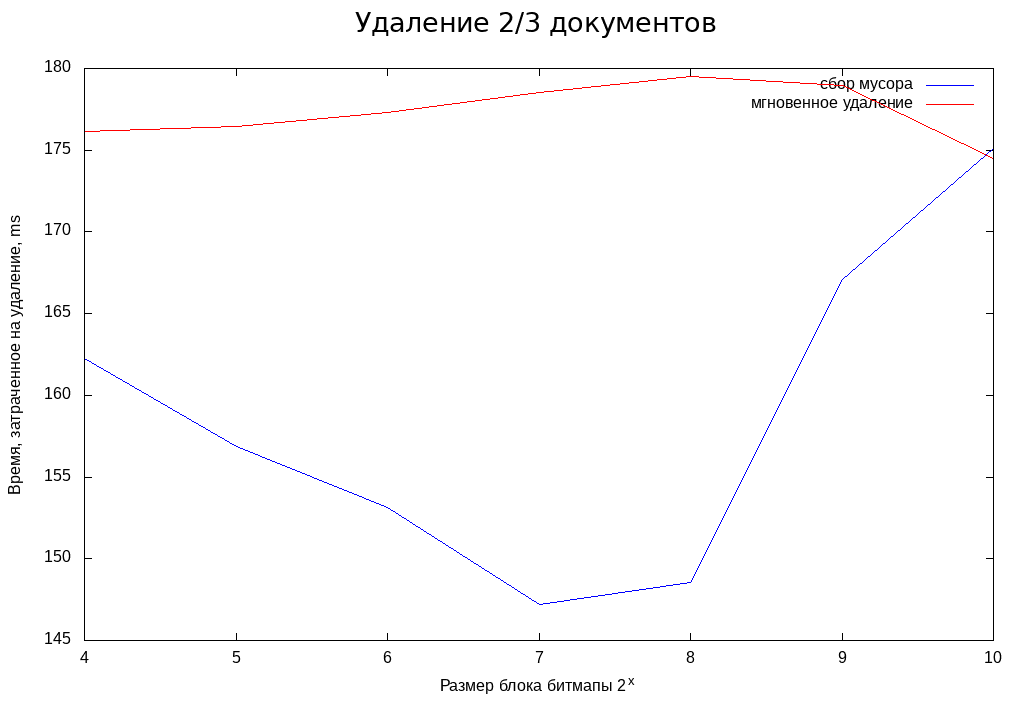
\includegraphics[width=\linewidth, height=10cm]{fig/time_1e3.png}
\end{figure}

\textbf{Вывод}: для $10^3$ элементов сбора мусора эффективнее по времени
выполнения, чем алгоритм <<мгновенного>> удаления. Предсказанное отличие
(см. с. ~\pageref{theory}) во времени работы видно невооруженным взглядом.

\subsubsection{Добавление $10^4$ документов, удаление $\frac{2}{3}$ документов}
\begin{figure}[H]
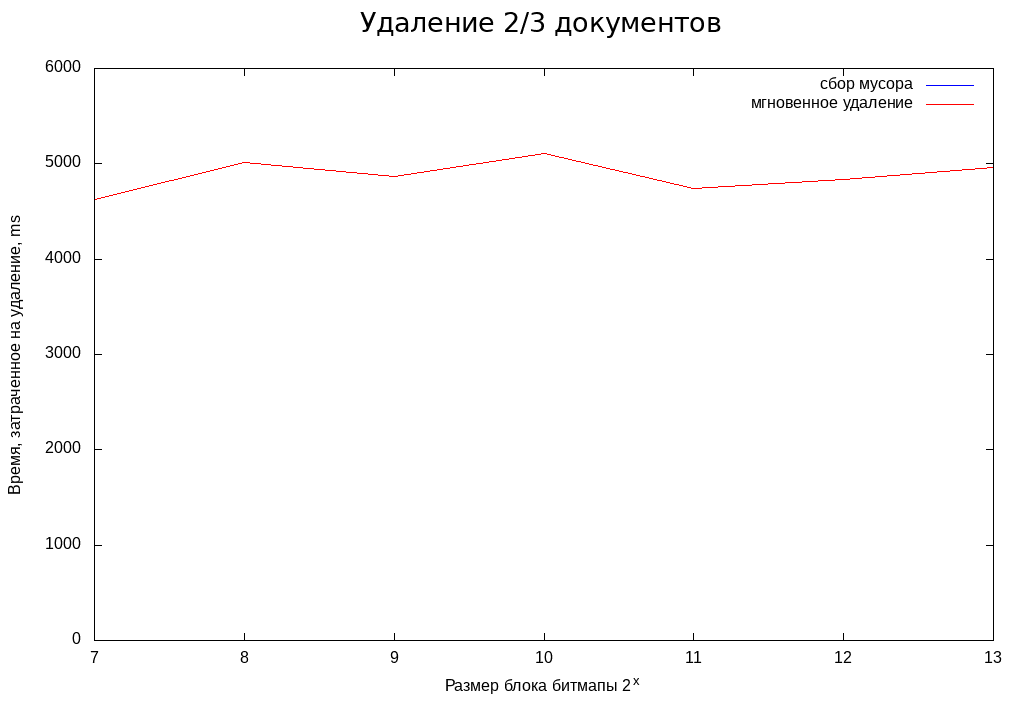
\includegraphics[width=\linewidth, height=11cm]{fig/time_1e4.png}
\end{figure}

\begin{table}[H]
      \caption{Время работы алгоритмов для $10^4$ документов, мс}
      \centering
      \small
      \singlespacing
      \begin{tabular}{|c|c|c|}
            \hline
            Размер блока & Сбор мусора                & <<Мгновенное удаление>> \\ \hline \hline
            7            & 2.70e-01	                  & 4.63e+03              \\ \hline
            8            & 2.72e-01	                  & 5.01e+03              \\ \hline
            9            & 2.77e-01	                  & 4.86e+03              \\ \hline
            10           & 2.54e-01                   & 5.11e+03              \\ \hline
            11           & 2.54e-01                   & 4.74e+03              \\ \hline
            12           & 2.54e-01	                  & 4.84e+03              \\ \hline
            13           & 2.54e-01	                  & 4.97e+03              \\ \hline
\end{tabular}
\end{table}

\textbf{Вывод}: для $10^4$ документов алгоритм становится в тысячи раз
эффективнее метода в лоб: <<мгновенного удаления>>, что соответствует выведенной теории.

\subsubsection{Добавление $10^5$ документов, удаление $\frac{2}{3}$ документов}

\begin{figure}[H]
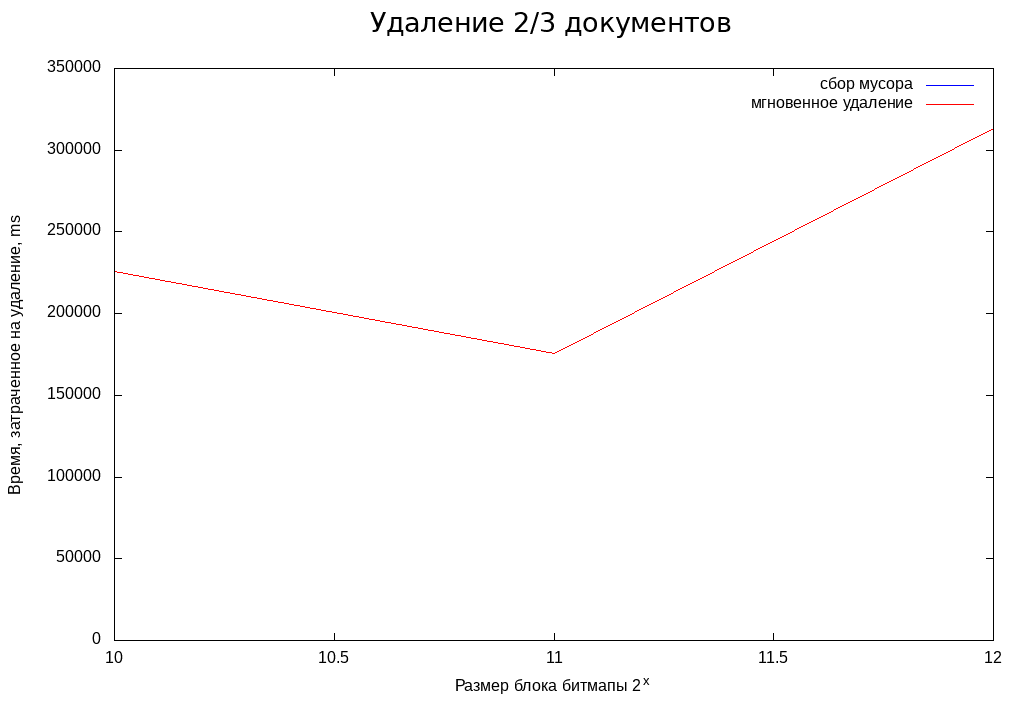
\includegraphics[width=\linewidth, height=11cm]{fig/time_1e5.png}
\end{figure}

\begin{table}[H]
      \caption{Время работы алгоритмов для $10^5$ документов, мс}
      \centering
      \small
      \singlespacing
      \begin{tabular}{|c|c|c|}
            \hline
            Размер блока & Сбор мусора                & <<Мгновенное>> удаление \\ \hline \hline
            10           & 2.54e-01                   & 2.26e+05              \\ \hline
            11           & 2.55e-01                   & 1.76e+05              \\ \hline
            12           & 2.54e-01                   & 3.14e+05              \\ \hline
            13           & 2.55e-01                   & 2.36e+05              \\ \hline
            14           & 2.55e-01                   & 2.33e+05              \\ \hline
            15           & 2.54e-01                   & 1.83e+05              \\ \hline
\end{tabular}
\end{table}

\textbf{Вывод}: для $10^5$ документов алгоритм становится в сотни тысяч раз
эффективнее метода в лоб: <<мгновенного удаления>>, что соответствует выведенной теории.

\subsubsection{Зависимость времени работы от числа документов}

\begin{figure}[H]
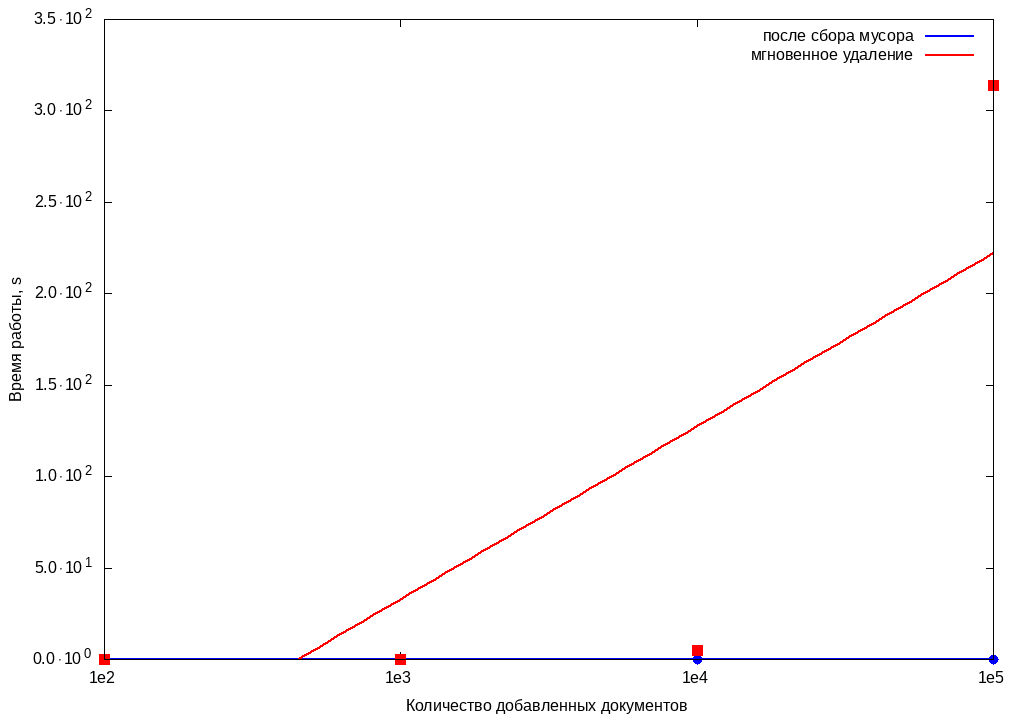
\includegraphics[width=\linewidth, height=11cm]{fig/time.png}
\end{figure}

\begin{table}[H]
      \caption{Время работы алгоритмов, с}
      \centering
      \small
      \singlespacing
      \begin{tabular}{|c|c|c|}
            \hline
            Число документов & Сбор мусора                & <<Мгновенное>> удаление \\ \hline \hline
            $10^2$           & 3.60e-02                   & 1.71e-02              \\ \hline
            $10^3$           & 1.47e-01                   & 1.79e-01              \\ \hline
            $10^4$           & 2.54e-04                   & 5.11e+00              \\ \hline
            $10^5$           & 2.54e-04                   & 3.14e+02              \\ \hline
\end{tabular}
\end{table}

\textbf{Вывод}: прослеживается глобальный тренд экспоненциального роста времени
работы алгоритма <<мгновенного>> удаления. График соответствует выведенной теории,
что позволяет еще раз указать на важность сбора мусора в данных.

\newpage
\subsection{Статистика количества операций записи, чтения и слияния для различного числа добавленных документов}

Во время выполнения тестов производительности на поиск элементов мы замеряли
некоторые статистические показатели: количество обращений в долгосрочную память
на жестком диске (операций чтения и записи), количество слияний с данными на
диске.
\subsubsection{Количество операций записи на диск}

\begin{figure}[H]
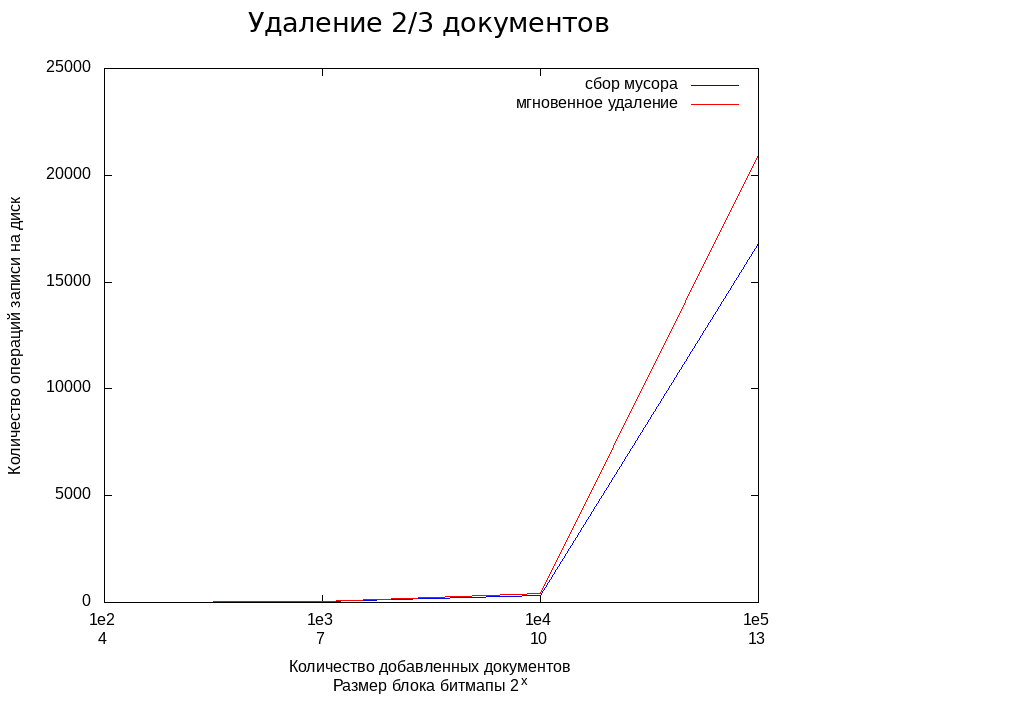
\includegraphics[width=\linewidth]{fig/writecalls.png}
\end{figure}

\begin{table}[H]
      \caption{Количество операций записи на диск}
      \centering
      \small
      \singlespacing
      \begin{tabular}{|c|c|c|}
            \hline
            Количество добавленных документов   & Сбор мусора                 & <<Мгновенное удаление>>     \\ \hline \hline
            100                                 & 8                           & 9                           \\ \hline
            1000                                & 38                          & 46                          \\ \hline
            10000                               & 347                         & 413                         \\ \hline
            100000                              & 14132                       & 11948                       \\ \hline
\end{tabular}
\end{table}

\subsubsection{Количество операций слияния с данными на диске}

\begin{figure}[H]
\centering
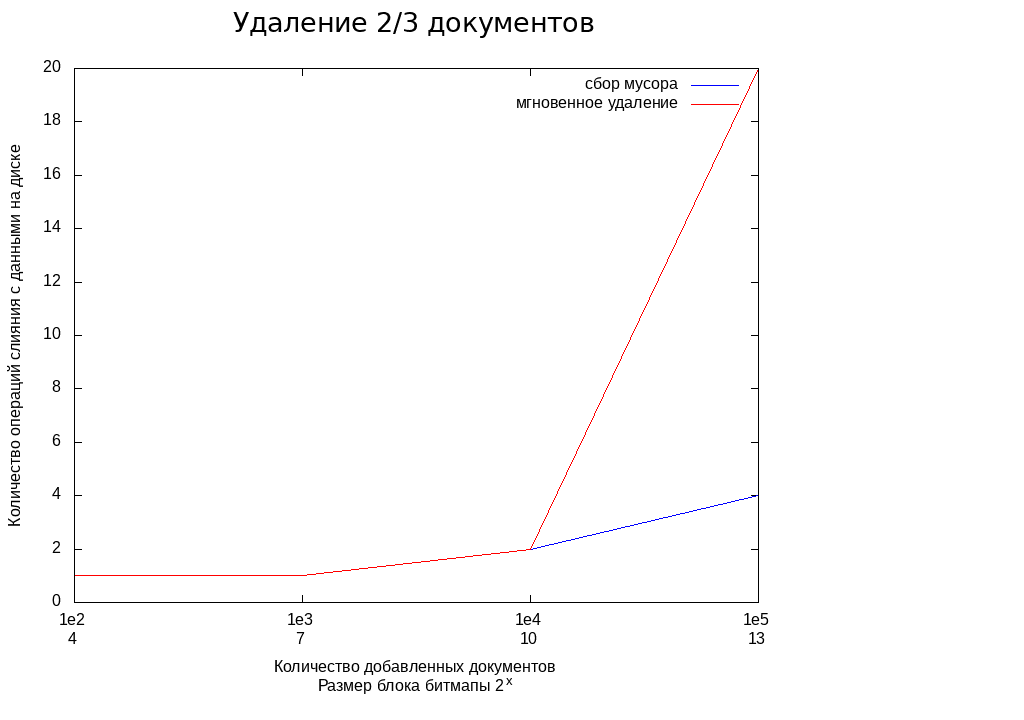
\includegraphics[width=\linewidth]{fig/merges.png}
\end{figure}

\begin{table}[H]
      \caption{Количество операций записи на диск}
      \centering
      \small
      \singlespacing
      \begin{tabular}{|c|c|c|}
            \hline
            Количество добавленных документов   & Сбор мусора                 & <<Мгновенное удаление>>     \\ \hline \hline
            100                                 & 1                           & 1                           \\ \hline
            1000                                & 1                           & 1                           \\ \hline
            10000                               & 2                           & 2                           \\ \hline
            100000                              & 4                           & 20                          \\ \hline
\end{tabular}
\end{table}

\textbf{Вывод}: алгоритм сбора мусора оказывается эффективнее в плане
обращений к <<медленной>> памяти по всем метрикам при увеличении размера 
обрабатываемых данных.
